\documentclass{article}
\usepackage[utf8]{inputenc}
\usepackage{amsmath}
\usepackage{float}
\usepackage{listings}
\usepackage[pdftex]{graphicx}
\usepackage{amssymb}
\usepackage{subcaption}
\usepackage{cancel}
\usepackage{float}
\usepackage{hyperref}
\DeclareMathOperator{\sech}{sech}

\newcommand{\pd}[2]{\frac{\partial{#1}}{\partial{#2}}}
%
\newcommand{\pdd}[2]{\frac{\partial^2{#1}}{\partial{#2}^2}}
%
\newcommand{\pddmixed}[3]{\frac{\partial^2{#1}}{\partial{#2}\partial{#3}}}

%---------------------------------------------------------
\author{Pratik Aghor}
\title{HW $\# 4$: Boundary Layer Analysis of Large $Re$ Flows}
\date{\today}  % Toggle commenting to test

\begin{document}

\maketitle
%----------------------------------------------
\section{$2d$ Laminar Jet:}
%----------------------------------------------
\begin{figure}[H]
    \centering
    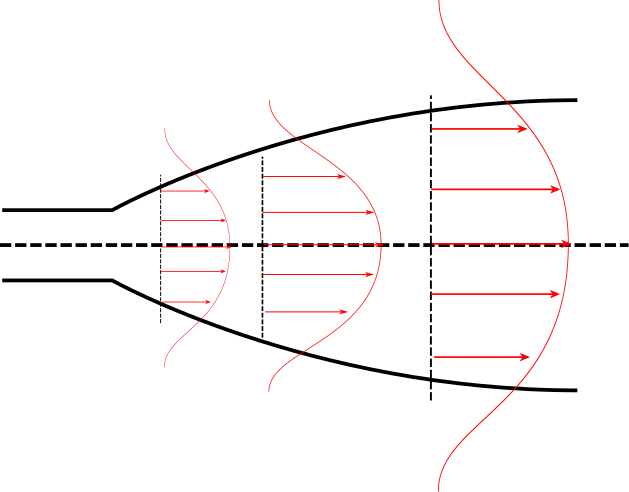
\includegraphics[scale = 0.3]{Figs/laminar_jet.png}
    \caption{Laminar Jet Sketch}
    \label{fig:laminar_jet}
\end{figure}

Governing equations are the $2d$ Navier-Stokes equations plus the continuity equation. 
%
\begin{align}\label{eq:NS_dim}
 \cancelto{0 \because \textrm{steady}}{\frac{\partial \underline{u}^{*} }{\partial t^{*}}} + [\underline{u}^{*} . \nabla^{*}] \underline{u}^{*} &= -\frac{1}{\rho^{*}}\cancelto{\frac{\partial p}{\partial y} \hat{e}_{y} \because \textrm{no imposed pressure gradient in x}}{\nabla^{*} p^{*}} + \nu^{*} {\nabla^{*}}^{2}\underline{u}^{*},\\
 %
 \nabla^{*} \cdot \underline{u}^{*} &= 0,
\end{align}
%
where stars denote dimensional quantities. We define the dimensionless quantities as follows:
$x = x^{*}/L, Y = y^{*}/\delta, u = u^{*}/U_{0}, V = v^{*}/V_{0}$, where $Y, V$ are the boundary layer variables. By continuity, $U_{0}/L \sim V_{0}/\delta$, or $\boxed{V_{0} = \epsilon U_{0}}$, with $\epsilon = \delta/L$. We now write the dimensional momentum equations inside the boundary layer (BL) and the relative sizes of terms.
%----------------------------------------------
\subsection{Laminar Jet - Scaling}
%----------------------------------------------

\begin{align}\label{eq:jet-x-mom-scaling}
 \begin{split}
  & u^{*}\frac{\partial u^{*}}{\partial x^{*}} + v^{*} \frac{\partial u^{*}}{\partial y^{*}} = \nu^{*}  \left[ \frac{\partial^{2} u}{\partial x^{2}} + \frac{\partial^{2} u}{\partial Y^{2}}\right]\\
  %
  & \frac{U_{0}^{2}}{L} \quad \quad \quad \frac{U_{0}^{2}}{L} \quad \quad \quad  \frac{\nu ^{*}U_{0}}{L^{2}} \quad \quad  \frac{\nu ^{*}U_{0}}{\epsilon^{2} L^{2}}\\
  %
  & 1 \quad \quad \quad \quad 1 \quad \quad \quad \quad \frac{1}{Re} \quad \quad \quad \frac{1}{\epsilon^{2} Re}
 \end{split}
\end{align}
%
Since physically, we know there is diffusion of vorticity in the $y$ direction and we can see that $ \frac{\partial^{2} u}{\partial Y^{2}} \gg \frac{\partial^{2} u}{\partial x^{2}} $, for keeping the diffusion term at the leading order, we must have $\epsilon \sim O( \frac{1}{\sqrt{Re}} )$. We choose $\boxed{\epsilon = \frac{1}{\sqrt{Re} } }$. Hence, the dimensionless $x$-momentum equation at the leading order takes the following form:
\begin{equation}\label{eq:jet-x-mom-dimless}
 u \frac{\partial u}{\partial x} + V \frac{\partial u}{\partial Y} = \frac{\partial^{2} u}{\partial Y^{2}}. 
\end{equation}
%
Let us do a similar scaling analysis for the $y$-moementum equation:

\begin{align}\label{eq:jet-y-mom-scaling}
 \begin{split}
  & u^{*}\frac{\partial v^{*}}{\partial x^{*}} + v^{*} \frac{\partial v^{*}}{\partial y^{*}} = -\frac{1}{\rho^{*}}\frac{\partial p^{*} }{\partial Y^{*}} + \nu^{*}  \left[ \frac{\partial^{2} v}{\partial x^{2}} + \frac{\partial^{2} v}{\partial Y^{2}}\right]\\
  %
  & \frac{\epsilon U_{0}^{2}}{L} \quad \quad \quad \frac{\epsilon U_{0}^{2}}{L} \quad \quad \quad  \frac{1}{\rho^{*}}\frac{P}{\epsilon L}\quad \quad \quad \frac{\epsilon \nu ^{*}U_{0}}{L^{2}} \quad \quad  \frac{\cancel{\epsilon} \nu ^{*}U_{0}}{\epsilon^{\cancel{2} } L^{2}}\\
  %
  & 1 \quad \quad \quad \quad 1 \quad \quad \quad \frac{P^{*}}{\epsilon^{2}\rho^{*} U_{0}^{2}} \quad \quad \quad \quad \quad \frac{1}{Re} \quad \quad \quad \frac{1}{\epsilon^{2} Re}\\
  %
  & 1 \quad \quad \quad \quad 1 \quad \quad \quad \frac{1}{\epsilon^{2}} \quad \quad \quad \quad \quad \quad \quad \frac{1}{Re} \quad \quad \quad 1\\
 \end{split}
\end{align}
choosing $P^{*} = \rho U_{0}^{2}$, we see that at the leading order, the dimensionless $y$-momentum equation reads:
\begin{equation}\label{eq:jet-y-mom-dimless}
 \frac{\partial p}{\partial y} = 0.
\end{equation}
%
This says that the outer pressure is simply impressed inside the BL, which is often the case in BL analyses. Hence, writing the dimensional governing equations:
\begin{align}\label{eq:jet-gov-eqns-dimless}
 \begin{split}
   u \frac{\partial u}{\partial x} + V \frac{\partial u}{\partial Y} &= \frac{\partial^{2} u}{\partial Y^{2}}\\
   %
    \frac{\partial u}{\partial x} + \frac{\partial V}{\partial Y} &= 0.
 \end{split}
\end{align}
%
%----------------------------------------------
\subsection{Laminar Jet - Conservation of momentum flux}
%----------------------------------------------

Now, the LHS of the $x$-momentum equation (Eqn. \ref{eq:jet-x-mom-dimless}) can be modified as follows:
\begin{equation}\label{eq:jet-modified-x-mom-dimless}
 \frac{\partial (u^{2})}{\partial x} - u \cancel{\frac{\partial u}{\partial x}} + \frac{\partial Vu}{\partial Y} - u \cancel {\frac{\partial V}{\partial Y}} = \frac{\partial^{2} u}{\partial Y^{2}}
\end{equation}
%
In modifying the LHS, we have used the incompressibility of the jet. Integrating Eqn.(\ref{eq:jet-modified-x-mom-dimless}) and using the boundary and symmetry conditions, we obtain:

\begin{align}\label{eq:jet-mom-flux-cons}
 \begin{split}
  & \int_{-\infty}^{\infty}\left[ \frac{\partial (u^{2})}{\partial x} dY + \frac{\partial Vu}{\partial Y} = \frac{\partial^{2} u}{\partial Y^{2}} \right] dY, \\
  %
  & \frac{\partial }{\partial x}\left[ \int_{-\infty}^{\infty} u^{2} dY \right] + \cancelto{0 }{\left[ Vu\right]}_{-\infty}^{\infty} = \cancelto{0 \because \textrm{ symmetry wrt } Y = 0}{\frac{\partial u}{\partial Y}\bigg|_{-\infty}^{\infty}},\\
  %
  & \boxed{\int_{-\infty}^{\infty} u^{2} dY = M},
 \end{split}
\end{align}
%
where $M$ does not vary along the streamwise direction $x$. 
%----------------------------------------------
\subsection{Laminar Jet - Similarity Solution:}
%----------------------------------------------
Since there are no imposed length or time-scales, there is a possibility that a similarity solution might exist. First, we introduce a stream-function
$\psi$, such that $u = \psi_{Y}, v = -\psi_{x}$. The incompressibility is automatically satisfied and the $x$-momentum equation becomes:
\begin{equation}\label{eq:jet-streamfn-x-mom-dimless}
 \psi_{Y} \psi_{xY} - \psi_{x}\psi_{YY} = \psi_{YYY}.
\end{equation} 
%
We now introduce the similarity ansatz:
\begin{equation}\label{eq:jet-similarity-ansatz}
 \psi (x, Y) = F(x) f(\eta), 
\end{equation}
with $\eta = Y/g(x)$. Substituting Eqn.(\ref{eq:jet-similarity-ansatz}) into Eqn.(\ref{eq:jet-mom-flux-cons}), we get a relationship between $F(x)$ and $g(x)$.
\begin{align}
 \begin{split}
 & \int_{-\infty}^{\infty}(\psi_{Y})^{2} dY = M \\
 & \int_{-\infty}^{\infty} F^{2} f'^{2} \cdot \left(\frac{\partial \eta}{\partial Y} \right)^{2} \cdot g d\eta = M\\
 & \frac{F(x)^{2}}{g(x)} \int_{-\infty}^{\infty} f'^{2}d\eta = M,
 \end{split}
\end{align}
here, primes denote differentiation wrt $\eta$. 
As suggested in the problem, setting $\int_{-\infty}^{\infty} f'^{2}d\eta = 2/3$ gives
$\boxed{F(x) = \left(\frac{3M}{2}\right)^{1/2} [g(x)]^{1/2}}$.

Now, we want to substitute Eqn.(\ref{eq:jet-similarity-ansatz}) into Eqn.(\ref{eq:jet-streamfn-x-mom-dimless}), but before doing so, we evaluate the specific derivatives. Note, we treat $x$ and $\eta$ as independent variables. Dots represent derivatives wrt $x$ and primes represent differentiation wrt $\eta$. 
\begin{align}
 \begin{split}
  & \psi_{X} = \left(\frac{3M}{2}\right)^{1/2} \cdot \frac{1}{2} g^{-1/2} \dot{g} \cdot f\\
  %
  & \psi_{Y} = \frac{F}{g} f' =  \left(\frac{3M}{2}\right)^{1/2} \frac{f'}{g^{1/2}},\\
  %
  & \psi_{YY} = \partial_{Y}\left(\left(\frac{3M}{2}\right)^{1/2} \frac{f'}{g^{1/2}} \right) =\left(\frac{3M}{2}\right)^{1/2} \frac{f''}{g^{3/2}},\\
  %
  & \psi_{YYY} = \partial_{Y}\left(\left(\frac{3M}{2}\right)^{1/2} \frac{f''}{g^{3/2}} \right) = \left(\frac{3M}{2}\right)^{1/2} \frac{f'''}{g^{5/2}}.
 \end{split}
\end{align}
Substituting these in Eqn.(\ref{eq:jet-streamfn-x-mom-dimless}) and canceling common factors, we obtain:
\begin{equation}
 -\frac{1}{2} \left(\frac{3M}{2}\right)^{1/2} f'^{2} \dot{g} - \frac{1}{2}\left(\frac{3M}{2}\right)^{1/2} \dot{g} f f' = f''' g^{-1/2}.
\end{equation}
%
To make the above equation independent of $x$, we must have $\dot{g} \sim g^{-1/2}$, which can be easily integrated to yield $\boxed{g(x) \sim x^{2/3} }$. As suggested in the problem, choosing $\boxed{ g(x) = \left(\frac{3M}{2}\right)^{-1/3}(3x)^{2/3} }$, the above equation reduces to:
\begin{equation}\label{eq:f-eqn}
 f'^{2} + f f'' + f''' = 0.
\end{equation}
%
The BC $u =0$ as $y \rightarrow \pm \infty$ reduces to $\boxed{f'(\infty) = 0}$. The symmetry condition at $Y=0$, $\frac{du}{dY} = 0$ reduces to $\boxed{f''(0) = 0}$. Also, by symmetry, we set the $\psi = 0$ streamline at $Y=0$, giving us another required BC $\boxed{f(0) = 0}$. 

Combining $ff'' + f'^{2} = (ff')'$, we get\
\begin{equation}
 f''' + (ff')' = 0
\end{equation}
Integrating once wrt $\eta$, obtain $f'' + ff' = c_{1}$. Since $f''(0) = f(0) = 0$, $\boxed{c_{1} = 0}$. Rewriting $f'' + ff' = 0$ as $f'' + \left(\frac{f^{2}}{2}\right)' = 0$ and integrating once more in $\eta$, 
\begin{equation}
 f'+ \frac{f^{2}}{2} = c_{2}.
\end{equation}
Solving this
\begin{equation}
 f(\eta) = 2A \tanh{A(\eta + k)}
\end{equation}
Since $f(0) = 0$, $\tanh{A(k)} = 0$, giving $\boxed{k = 0}$ $\Rightarrow \boxed{f(\eta) = 2A \tanh{(A\eta)}}  $.\\
%
We had set $\int_{-\infty}^{\infty} f'^{2}d\eta = 2/3$. This yields,
\begin{align}
 \begin{split}
  & \int_{-\infty}^{\infty} f'^{2}d\eta = 2/3, \\
  %
  & 4 A^{4} \int_{-\infty}^{\infty} \sech^{4}{(A\eta)}d\eta = 2/3,\\
  %
  &\frac{2A^{4}}{A}\int_{-\infty}^{\infty} \sech^{4}{\zeta} d\zeta = 1/3,\\
  %
  & 2 A^{3} \cdot 4/3 = 1/3\\
  & \boxed{A = 1/2}.
 \end{split}
\end{align}
%
Now, we can obtain $u(x, Y)$ as follows:
\begin{align}
 \begin{split}
  & u = \psi_{Y} =  \left(\frac{3M}{2}\right)^{1/2} \frac{f'}{g^{1/2}}, \\
  %
  & \boxed{u =\frac{1}{2}\left(\frac{3M^{2}}{4x}\right)^{1/3}\sech^{2}{(\eta/2)} }.
 \end{split}
\end{align}
\begin{figure}[H]
    \centering
    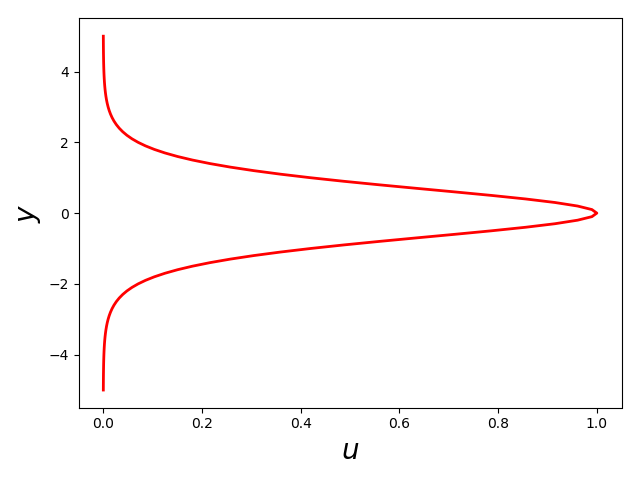
\includegraphics[scale = 0.8]{Figs/laminar_jet_profile.png}
    \caption{Numerical plotting of $\sech^{2}(y)$, assume $x = 1$.}
    \label{fig:laminar_jet}
\end{figure}

%----------------------------------------------
\section{Quasi-Geostrophic (QG) Vorticity Equation, Ekman Boundary Layer (BL) in the $\beta$-Plane:}
%----------------------------------------------
From our discussion of Ekman boundary layers that the leading-order interior geostrophic flow ($u_{0}$ and $v_{0}$) is not constrained at leading order; that is, $u_{0}$ and $v_{0}$ are in geostrophic balance with the leading order interior pressure $\pi_{0}$, but these variables are otherwise unknown. This indeterminacy can be remedied by going to the next order in the expansion for the interior flow and making use of our leading-order Ekman boundary layer analysis.
%----------------------------------------------
\subsection{The $\beta$-Plane:}
%----------------------------------------------
\begin{figure}[H]
    \centering
    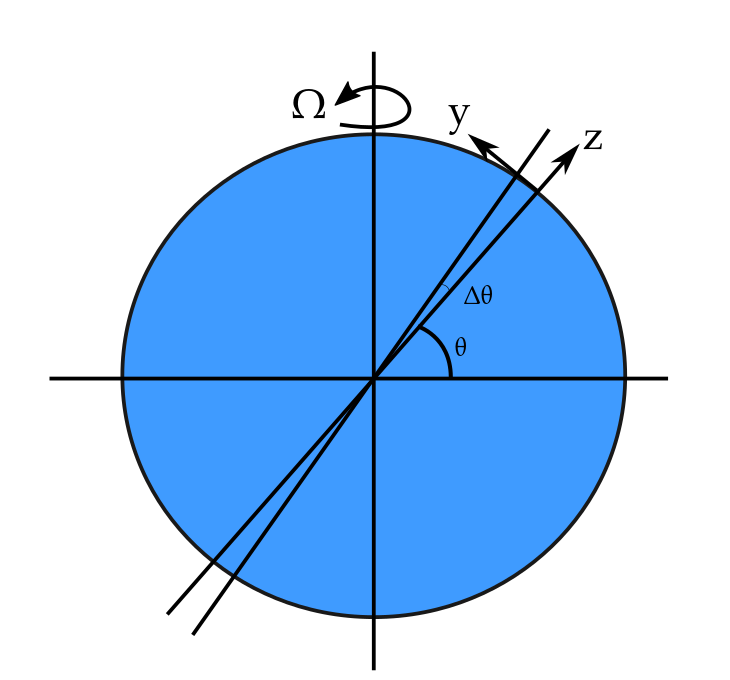
\includegraphics[scale = 0.3]{Figs/beta_plane.png}
    \caption{The $\beta$-plane approximation}
    \label{fig:beta_plane}
\end{figure}

The ``Coriolis parameter'' $f$ is given by (twice) the component of the planetary angular velocity in the local $z$-direction. We measure $\theta$ from the equator, so $\theta=0$ corresponds to the equator while at the North pole, $\theta=\pi/2$. 
\begin{align}\label{eq:beta-plane-approx}
 \begin{split}
  & f = 2\Omega \sin{\theta},\\
  %
  & f = 2\Omega \sin{\theta_{0}} + (\Delta \theta) 2\Omega \cos{\theta_{0}} + \textrm{h.o.t.},\\
  %
  &\textrm{noting } r_{0} \Delta \theta = \tilde{y},\\
  %
  & f \approx 2\Omega \sin{\theta_{0}} + \frac{\tilde{y}}{r_{0}} 2\Omega \cos{\theta_{0}},\\
  %
  & \boxed{ f \approx f_{0} + \beta_{0} \tilde{y}},
 \end{split}
\end{align}
where $f_{0} = 2\Omega \sin{\theta_{0}}, \beta_{0} = \frac{2\Omega \cos{\theta_{0}}}{r_{0}}$ are dimensional parameters and $\tilde{y}$ is the local cross-flow (northward) co-ordinate (we assume that the wind is blowing in the $x$-direction).  
%----------------------------------------------
\subsection{Governing Equations:}
%----------------------------------------------
\begin{figure}[H]
    \centering
    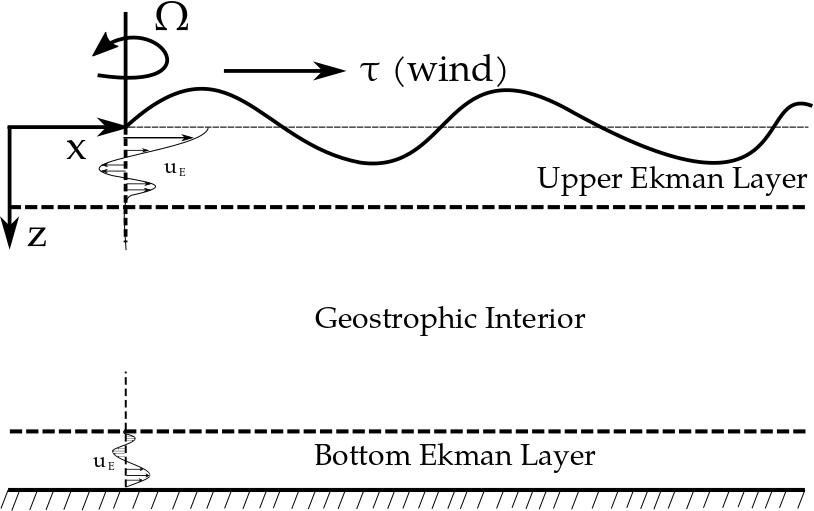
\includegraphics[scale = 0.5]{Figs/ekman_layers.png}
    \caption{Sketch of Ekman layers at the top and bottom. The flow in the interior is geostrophic.}
    \label{fig:ekman_layers}
\end{figure}

\begin{align}\label{eq:rotating-NS}
 \begin{split}
  & \pd{u}{t} + u \pd{u}{x} + v \pd{u}{y} + w\pd{u}{z} - fv = -\frac{1}{\rho} \pd{\pi}{x} + \nu\left[\pdd{u}{x} + \pdd{u}{y} + \pdd{u}{z}\right],\\
  %
  & \pd{v}{t} + u \pd{v}{x} + v \pd{v}{y} + w\pd{v}{z} + fu = -\frac{1}{\rho} \pd{\pi}{y} + \nu\left[\pdd{v}{x} + \pdd{v}{y} + \pdd{v}{z}\right],\\
  %
  & \pd{w}{t} + u \pd{w}{x} + v \pd{w}{y} + w\pd{w}{z}  = -\frac{1}{\rho} \pd{\pi}{z} + \nu\left[\pdd{w}{x} + \pdd{w}{y} + \pdd{w}{z}\right],\\
  %
  & \pd{u}{x} + \pd{v}{y} + \pd{w}{z} = 0.
 \end{split}
\end{align}
 First, let us look at the Coriolis terms. For example, take $fu$. 
\begin{equation}
 f u = (f_{0}+\beta_{0}\tilde{y})u = f_{0}U_{0}\left(1 + \frac{\beta_{0} L}{f_{0}} y \right)u 
\end{equation}
where $y$ and $U$ on the RHS are dimensionless terms. Simplifying further and taking only the dimensionless version now, 
\begin{equation}
 \left(1 + \frac{\beta_{0} L}{f_{0}} y \right)u  = \bigg(1 + \underbrace{ \frac{\beta_{0} L^{2}}{U_{0}} }_{\beta} \underbrace{ \frac{U_{0}}{L f_{0}} }_{\epsilon} y \bigg)u = (1 + \epsilon \beta y) u, 
\end{equation}
where $\beta =  \frac{\beta_{0} L^{2}}{U_{0}} $ is a new parameter and $\epsilon =  \frac{U_{0}}{L f_{0}}$ is the familiar Rossby number.\\
%
We scale $x, y \sim L, z \sim D, f\sim f_{0}, t\sim L/U_{0}, u, v \sim U_{0}, w \sim W_{0}$. From continuity, it is immediately clear that $\frac{W_{0}}{D} \sim \frac{U_{0}}{L}$ or $W_{0} \sim \Gamma U_{0}$, where $\Gamma = \frac{D}{L}$ is the aspect ratio. \\
%
Let $p \sim P$. For geostrophic balance at the leading order, $\frac{1}{\rho} \frac{\partial \pi}{\partial x} \sim f v$, yielding $\boxed{P = \rho f_{0} U_{0} L}$.
%
Using these scalings, let us non-dimensionalize the $x$-momentum equation:
\begin{align}
 \begin{split}
  & \pd{u}{t} + u \pd{u}{x} + v \pd{u}{y} + w\pd{u}{z} - fv = -\frac{1}{\rho} \pd{\pi}{x} + \nu\left[\pdd{u}{x} + \pdd{u}{y} + \pdd{u}{z}\right],\\
  %
  &\frac{U_{0}^{2}}{L} \quad \quad \frac{U_{0}^{2}}{L} \quad \quad  \frac{U_{0}^{2}}{L} \quad \quad \frac{U_{0}^{2}}{L} \quad f_{0}U_{0} \quad f_{0}U_{0} \quad \frac{\nu \Gamma^{2}U_{0}}{D^{2}} \quad \frac{\nu \Gamma^{2}U_{0}}{D^{2}} \quad \frac{\nu U_{0}}{D^{2}} \\
  & \epsilon \qquad \qquad \epsilon \qquad\epsilon \qquad \qquad \epsilon \qquad 1 \qquad 1 \qquad \qquad \Gamma^{2}E \qquad  \Gamma^{2}E \qquad  E 
 \end{split}
\end{align}
Here, we divided throughout by $f_{0}U_{0}$ to get the coefficients. In the above $\epsilon = \frac{U_{0}}{Lf_{0}}$ is the Rossby number, while $E = \frac{\nu}{f_{0}D_{0}^{2}}$ is the Ekman number. We can do similar analyses for other momenum equations. The governing dimensionless equations now become:
\begin{align}\label{eq:rotating-NS-dimless}
 \begin{split}
  \epsilon \left[\pd{u}{t} + u \pd{u}{x} + v \pd{u}{y} + w\pd{u}{z}\right] - (1 + \beta \epsilon y)v &= -\pd{\pi}{x} + \Gamma^{2}E\left[\pdd{u}{x} + \pdd{u}{y}\right] + E \pdd{u}{z},\\
  %
  \epsilon \left[\pd{v}{t} + u \pd{v}{x} + v \pd{v}{y} + w\pd{v}{z}\right] + (1 + \beta \epsilon y)u &= -\pd{\pi}{y} + \Gamma^{2}E\left[\pdd{v}{x} + \pdd{v}{y}\right] + E \pdd{v}{z},\\
  %
  \Gamma^{2} \epsilon \left[\pd{w}{t} + u \pd{w}{x} + v \pd{w}{y} + w\pd{w}{z} \right] &= - \pd{\pi}{z} + \Gamma^{4}E\left[\pdd{w}{x} + \pdd{w}{y}\right] + \Gamma^{2}E \pdd{w}{z},\\
  %
  \pd{u}{x} + \pd{v}{y} + \pd{w}{z} &= 0.
 \end{split}
\end{align}
%----------------------------------------------
\subsection{``Outer'' Interior Solution:}
%----------------------------------------------
As suggested in the problem writing $\underline{u} = \underline{u}_{0} + \epsilon \underline{u}_{1} + \hdots$ and $\pi = \pi_{0} + \epsilon \pi_{1} + \hdots$, substituting in Eqn. (\ref{eq:rotating-NS-dimless}), collecting terms at different powers of $\epsilon$, we get:
\begin{align}\label{eq:order-1-outer}
 \begin{split}
 O(1):& \textrm{Geostrophic balance:} \\
 %
 & \pd{\pi_{0}}{x} = v_{0}, \\
 & \pd{\pi_{0}}{y} = -u_{0}, \\
 & \pd{\pi_{0}}{z} = 0,\\
 & \pd{u_{0}}{x} + \pd{v_{0}}{y} + \pd{w_{0}}{z} = 0.\\
 \textrm{BCs}:& u_{0} = v_{0} = w_{0} = 0 \quad \textrm{at} \quad z = -1, \\
 & w_{0} = 0 \quad \textrm{at} \quad z = 0 \\
 & \pd{u_{0}}{z} = \frac{\tau}{\sqrt{E}} \quad \textrm{at} \quad z = 0, \\
 & \pd{v_{0}}{z} = 0 \quad \textrm{at} \quad z = 0, \\
 \end{split}
\end{align}
where $\tau$ is the dimensionless wind-shear at the free surface. The system is not closed, since there is no way of determining $\pi_{0}$ from the current equations. However, we can still draw some conclusions from the leading order geostrophic balance. Substituting the $x$- and $y$- geostrophic balance equations into continuity, we see $-\cancel{\pddmixed{\pi_{0}}{x}{y}} + \cancel{\pddmixed{\pi_{0}}{y}{x}} + \pd{w_{0}}{z} = 0$. This shows that $w_{0}$ is independent of $z$ or $\boxed{w_{0}\equiv w_{0}(x, y, t)}$.\\
%
Taking the $z$-derivative of the $x$- and $y$-geostrophic balance equations and using the fact that $\pd{\pi_{0}}{z} = 0$, we obtain $\pd{u_{0}}{z} = \pd{v_{0}}{z} = 0$. That is, $u_{0}$ and $v_{0}$ are also independent of $z$ or  $\boxed{[u_{0}, v_{0}]\equiv [u_{0}, v_{0}](x, y, t)}$. Now, we go to the next order. Using the distinguished limit, we had related in the two small parameters $\epsilon$ and $E$, such that $ r = \frac{\sqrt{E}}{\epsilon} = O(1)$ as $\epsilon \rightarrow 0$. Keeping this in mind, we write the $O(\epsilon)$ equations as follows:
\begin{align}\label{eq:order-eps-outer}
 \begin{split}
 O(\epsilon):& \\
 %
 & \pd{u_{0}}{t} + u_{0}\pd{u_{0}}{x} + v_{0}\pd{u_{0}}{y} + w_{0}\pd{u_{0}}{z} - v_{1} - \beta y v_{0} = -\pd{\pi_{1}}{x}, \\
 %
 & \pd{v_{0}}{t} + u_{0}\pd{v_{0}}{x} + v_{0}\pd{v_{0}}{y} + w_{0}\pd{v_{0}}{z} + u_{1} + \beta y u_{0} = -\pd{\pi_{1}}{y}, \\
 &%
 \Gamma^{2} \left[ \pd{w_{0}}{t} + u_{0}\pd{w_{0}}{x} + v_{0}\pd{w_{0}}{y} + w_{0}\pd{w_{0}}{z} \right] = -\pd{\pi_{1}}{z}, \\
 %
 &\pd{u_{1}}{x} + \pd{v_{1}}{y} + \pd{w_{1}}{z} = 0.\\
  \textrm{BCs}:& u_{1} = v_{1} = w_{1} = 0 \quad \textrm{at} \quad z = -1, \\
 & w_{1} = 0 \quad \textrm{at} \quad z = 0 \\
 & \pd{u_{1}}{z} = 0 \quad \textrm{at} \quad z = 0, \\
 & \pd{v_{1}}{z} = 0 \quad \textrm{at} \quad z = 0. \\
 \end{split}
\end{align}
%
To eliminate pressure, cross differentiating the $x$- and $y$- moementum equations and subtracting, we obtain:
\begin{align}\label{eq:qg_vorticity}
 \begin{split}
  & \pd{}{x}\left[\pd{v_{0}}{t} + u_{0}\pd{v_{0}}{x} + v_{0}\pd{v_{0}}{y} + w_{0}\pd{v_{0}}{z} + u_{1} + \beta y u_{0} = -\pd{\pi_{1}}{y}\right]\\
  %
  -&\pd{}{y}\left[ \pd{u_{0}}{t} + u_{0}\pd{u_{0}}{x} + v_{0}\pd{u_{0}}{y} + w_{0}\pd{u_{0}}{z} - v_{1} - \beta y v_{0} = -\pd{\pi_{1}}{x}\right]\\
  & --------------------------- \\
  %
  & \pd{\omega_{z0}}{t} + u_{0}\pd{\omega_{z0}}{x} + v_{0}\pd{\omega_{z0}}{y} + w_{0}\pd{\omega_{z0}}{z} + \underbrace{\left( \pd{u_{1}}{x} + \pd{v_{1}}{y}\right)}_{-\pd{w_{1}}{z}} + \beta y \bigg( \cancel{\pd{u_{0}}{x} + \pd{v_{0}}{y}}\bigg) + \beta v_{0} = 0,\\
  %
  & \boxed{\frac{D\omega_{z0}}{Dt} + \beta v_{0} = \pd{\omega_{z0}}{t} + u_{0}\pd{\omega_{z0}}{x} + v_{0}\pd{\omega_{z0}}{y} + w_{0}\pd{\omega_{z0}}{z} + \beta v_{0} = \pd{w_{1}}{z} }.
 \end{split}
\end{align}
Here $\boxed{\omega_{z0} = \pd{v_{0}}{x} - \pd{u_{0}}{y}}$ is the leading-order (\textit{relative}) vertical vorticity. Copying the comment from the assignment here for completion.
``Physically, $\omega_{z0}$ is the leading-order relative z-vorticity: the total z-vorticity equals the sum of $\omega_{z0}$ plus $\epsilon^{-1}$ , where in dimensional terms ``$\epsilon^{-1}$''
corresponds to $f_{0} \equiv 2\Omega \sin{\theta_{0}}$, i.e. the $z$-vorticity fluid particles acquire simply because they are rotating with the Earth. Thus, in terms of vorticity dynamics, the right-hand-side of Eqn.(\ref{eq:qg_vorticity}) is a vortex-stretching term; more specifically, stretching of planetary vortex tubes by the difference in vertical velocities at the ends of these vertically-oriented tubes. (The term involving $\beta$ physically represents the advection of planetary vortex tubes.)''\\
%
To close Eqn.(\ref{eq:qg_vorticity}), we integrate it across the basin. Noting that $u_{0}, v_{0}$(and hence, $\omega_{z0}$) as well as $w_{0}$ are independent of $z$, we get:
\begin{equation}\label{eq:qg-half-done}
 \boxed{\frac{D\omega_{z0}}{Dt} + \beta v_{0} = \pd{\omega_{z0}}{t} + u_{0}\pd{\omega_{z0}}{x} + v_{0}\pd{\omega_{z0}}{y} + w_{0}\pd{\omega_{z0}}{z} + \beta v_{0} = w_{1}\big|_{z=0} - w_{1}\big|_{z=-1} }.
\end{equation}
%
To find the RHS, we must do matched asymptotics. 
%----------------------------------------------
\subsection{``Inner'' Solution at the Upper Free Surface:}
%----------------------------------------------
Redefining boundary layer variables as $\hat{u}, \hat{v}, \hat{w}, \hat{\pi}$ and the co-ordinates as $\hat{x} = x, \hat{y} = y, \hat{z}= z/h(\epsilon)$, where $h(\epsilon) = h^{*}/D$ is the dimensionless thickness of the BL, we obtain:

\begin{align}\label{eq:bl-rotating-NS-dimless}
 \begin{split}
  \epsilon \left[\pd{\hat{u} }{\hat{t} } + \hat{u} \pd{\hat{u} }{\hat{x} } + \hat{v} \pd{\hat{u} }{\hat{y} } + \frac{\hat{w}}{h}\pd{\hat{u}}{\hat{z} }\right] - (1 + \beta \epsilon \hat{y}) \hat{v} &= -\pd{\hat{\pi} }{\hat{x} } + \Gamma^{2}E\left[\pdd{\hat{u}}{\hat{x}} + \pdd{\hat{u}}{\hat{y}}\right] + \frac{E}{h^{2}} \pdd{\hat{u}}{\hat{z} },\\
  %
  \epsilon \left[\pd{\hat{v} }{\hat{t} } + \hat{u} \pd{\hat{v} }{\hat{x} } + \hat{v} \pd{\hat{v} }{\hat{y} } + \frac{\hat{w}}{h}\pd{\hat{v}}{\hat{z} }\right] + (1 + \beta \epsilon \hat{y}) \hat{u} &= -\pd{\hat{\pi} }{\hat{y} } + \Gamma^{2}E\left[\pdd{\hat{v}}{\hat{x}} + \pdd{\hat{v}}{\hat{y}}\right] + \frac{E}{h^{2}} \pdd{\hat{v}}{\hat{z} },\\
  %
  \Gamma^{2} \epsilon \left[\pd{\hat{w} }{\hat{t} } + \hat{u} \pd{\hat{w}}{\hat{x} } + \hat{v} \pd{\hat{w}}{\hat{y}} + \hat{w}\pd{\hat{w}}{\hat{z}} \right] &= - \frac{1}{h}\pd{\hat{\pi}}{\hat{z} } + \Gamma^{4}E\left[\pdd{\hat{w}}{\hat{x}} + \pdd{\hat{w}}{\hat{y}}\right] + \Gamma^{2}\frac{E}{h^{2}} \pdd{\hat{w}}{\hat{z}},\\
  %
  \pd{\hat{u}}{\hat{x}} + \pd{\hat{v}}{\hat{y}} + \frac{1}{h}\pd{\hat{w}}{\hat{z}} &= 0.
 \end{split}
\end{align}
In what follows, since $\hat{x} = x, \hat{y} = y$, we will drop the hats on the $x$ and $y$, but will keep the hat on $\hat{z}$ to remind ourselves that $\hat{z}$ is a BL variable. Before posing an asymptotic expansion and collecting terms, some observations are important. We first choose $h = O(\sqrt{E})$, specifically $h = \sqrt{E} = r\epsilon$, in order to keep the $\hat{z}$-diffusion at the leading order. This is the crucial physics that our interior, outer solution lacks. If we multiply through by $h = \epsilon$ the continuity equation, at leading order, we would obtain: $\boxed{\pd {\hat{w}_{0}}{\hat{z}} = 0}$, i.e., $\hat{w}_{0}$ is independent of $\hat{z}$. Using the upper surface BC, $\hat{w} = 0$ at $\hat{z} = 0$, we get $\hat{w}_{0} = 0$. Hence, the asymptotic sequence for $\boxed{\hat{w} \sim \epsilon \hat{w}_{1} + \hdots}$. \\
%
Now, posing $\hat{u} \sim \hat{u}_{0} + \epsilon \hat{u}_{1} + \hdots$, $\hat{v} \sim \hat{v}_{0} + \epsilon \hat{v}_{1} + \hdots$ and $\hat{\pi} \sim \hat{\pi}_{0} + \epsilon \hat{\pi}_{1} + \hdots$, collecting terms at leading order, we get the following (note: since the leading order in the $\hat{z}$-momentum equation is $O(1/h)$, multiply through by $h = r\epsilon$ and collect terms):

\begin{align}\label{eq:bl-order-1}
 \begin{split}
  & -\hat{v}_{0} = -\pd{\hat{\pi}_{0} }{x} + \pdd{\hat{u}_{0}}{\hat{z} },\\
  %
  &\hat{u}_{0} = -\pd{\hat{\pi}_{0} }{y} + \pdd{\hat{v}_{0}}{\hat{z} },\\
  %
  & 0 = \pd{\hat{\pi}}{\hat{z} }.
 \end{split}
\end{align}
We solve for $\hat{u}_{0}, \hat{v}_{0}$ by obtaining the homogeneous solution (with inhomogeneous BCs: $\frac{1}{\cancel{h} }\pd{\hat{u}_{H}}{\hat{z}} = \frac{\tau}{\cancel{\sqrt{E} }}$) and the inhomogeneous solution (with homogeneous BCs: $\pd{\hat{u}_{I}}{\hat{z}} = 0$). Defining:
\begin{align}
 \begin{split}
  &\hat{u}_{0} = \hat{u}_{H} + \hat{u}_{I}\\
  %
  &\hat{v}_{0} = \hat{v}_{H} + \hat{v}_{I}\\
 \end{split}
\end{align}
%
%----------------------------------------------
\subsubsection{Homogeneous Solution:}
%----------------------------------------------
The homogeneous part of Eqn.(\ref{eq:bl-order-1}) can be written as:
\begin{align}
 \begin{split}
  & -\hat{v}_{H} = \pdd{\hat{u}_{H}}{\hat{z} },\\
  %
  &\hat{u}_{H} = \pdd{\hat{v}_{H}}{\hat{z} }.\\
 \end{split}
\end{align}
%
The two equations can be combined into the form
\begin{equation}\label{eq:bl-complex-hom}
\pdd{\mathcal{U}_{H}}{\hat{z}} - i \mathcal{U}_{H} = 0,
\end{equation}
where $ \mathcal{U}_{H} = \hat{u}_{H} + i \hat{v}_{H}$. The solutions of Eqn.(\ref{eq:bl-complex-hom}) are 
\begin{equation}
 \mathcal{U}_{H} = A e^{\lambda \hat{z}}.
\end{equation}
%
Substituting into Eqn.(\ref{eq:bl-complex-hom}), we get $\lambda^{2} = i$, or $\lambda = \pm \frac{(1+i)}{\sqrt{2}}$. The general solution then becomes:
\begin{equation}\label{eq:bl-complex-hom-gen-soln}
 \mathcal{U}_{H} = A e^{\frac{(1+i)}{\sqrt{2}}\hat{z}} + B e^{-\frac{(1+i)}{\sqrt{2}}\hat{z}}.
\end{equation}
%
When matching with, we'd need to take the outer limit $\hat{z}\rightarrow -\infty$ of this inner solution. Hence, for consistency, we must have $\boxed{B = 0}$, giving 
%
\begin{equation}\label{eq:bl-complex-hom-upper}
 \mathcal{U}_{H} = A e^{\frac{(1+i)}{\sqrt{2}}\hat{z}}.
\end{equation}
As we wrote earlier, we'd impose the inhomogeneous BCs on the homogeneous solution. The BC for $\mathcal{U}_{H}$ at $\hat{z} = 0$ is obtained by combining BCs for $\hat{u}_{H}$ and $\hat{v}_{H}$, namely,
\begin{align}\label{eq:bl-complex-hom-upper-bc}
 \begin{split}
  &\frac{1}{\cancel{h} }\pd{\hat{u}_{H}}{\hat{z}}\bigg|_{\hat{z} = 0} = \frac{\tau}{\cancel{\sqrt{E} }},\\
  %
  & \pd{\hat{u}_{H}}{\hat{z}}\bigg|_{\hat{z} = 0} = \tau, \\
  %
  &\pd{\hat{v}_{H}}{\hat{z}}\bigg|_{\hat{z} = 0} = 0,\\
  %
  &\boxed{\pd{\mathcal{U}_{H}}{\hat{z}}\bigg|_{\hat{z} = 0} = \tau + i(0) }.\\
 \end{split}
\end{align}
This gives
\begin{align}
 \begin{split}
  & A \frac{(1+i)}{\sqrt{2}} = \tau, \\
  %
  & \boxed{A = \tau \frac{(1-i)}{\sqrt{2}} },\\
  %
  &\boxed{\mathcal{U}_{H} = \left[\frac{(\tau-i\tau)}{\sqrt{2}} \right] \exp{\left(\frac{(1+i)}{\sqrt{2}}\hat{z}\right)} }. 
 \end{split}
\end{align}
%
%----------------------------------------------
\subsubsection{Inomogeneous Solution:}
%----------------------------------------------
We can just read-off the inhomogeneous solution. 
\begin{align}\label{eq:bl-complex-inhom-upper}
 \begin{split}
  & \hat{u}_{I} = -\pd{\hat{\pi}_{0} }{y},\\
  %
  & \hat{v}_{I} = \pd{\hat{\pi}_{0} }{x},\\
  %
  &\boxed{\mathcal{U}_{I} = -\pd{\hat{\pi}_{0} }{y} + i \pd{\hat{\pi}_{0} }{x}}. 
 \end{split}
\end{align}
This is consistent since $\pd{\hat{\pi}_{0} }{z} = 0$. Consistency can be checked by substituting the inhomogeneous solution into Eqn.(\ref{eq:bl-order-1}). The inhomogeneous solution satisfies homogeneous BCs $ \pd{\hat{u}_{I}}{\hat{z}}\bigg|_{\hat{z} = 0} =  \pd{\hat{v}_{I}}{\hat{z}}\bigg|_{\hat{z} = 0} = 0$.\\
%
%----------------------------------------------
\subsubsection{Matching: Inner(Outer) $=$ Outer(Inner)}
%----------------------------------------------
\begin{itemize}
 \item Inner limit of the outer geostrophic flow (Eqn. \ref{eq:order-1-outer}):
 \begin{equation}
  \lim_{z \rightarrow 0} u_{0} + i v_{0} = - \pd{\pi_{0}}{y} + i \pd{\pi_{0}}{x}.
 \end{equation}
 %
 \item Outer limit of the inner BL flow:
 \begin{equation}
  \lim_{\hat{z} \rightarrow -\infty} \mathcal{U} = 0 - \pd{\hat{\pi}_{0}}{y} + i \pd{\hat{\pi}_{0}}{x}.
 \end{equation}
 %
\end{itemize}
%
Matching the two limits, we obtain
\begin{align}
 \begin{split}
   & \pd{\pi_{0}}{x} = \pd{\hat{\pi}_{0}}{x},\\
   %
   & \pd{\pi_{0}}{y} = \pd{\hat{\pi}_{0}}{y}. \\
   %
   & \Rightarrow \boxed{\pd{\hat{\pi}_{0}}{x} = v_{0} }\textrm{ and }\\
   %
   & \boxed{ -\pd{\hat{\pi}_{0}}{y} = u_{0}}.   
 \end{split}
\end{align}
%
Substituting these into the BL solution and writing in terms of components, we get
%
\begin{align}\label{eq:bl-full-soln-order-1}
 \hat{u}_{0} \hat{e}_{x} + \hat{v}_{0} \hat{e}_{y} &= \left\{ u_{0} + \frac{\tau}{\sqrt{2}} \exp{\left(\frac{\hat{z}}{\sqrt{2}}\right)} \left[\cos{\left(\frac{\hat{z}}{\sqrt{2}} \right)} + \sin{\left(\frac{\hat{z}}{\sqrt{2}} \right)} \right] \right\}\hat{e}_{x} \\
 %
 &+ \left\{ v_{0} + \frac{\tau}{\sqrt{2}} \exp{\left(\frac{\hat{z}}{\sqrt{2}}\right)} \left[\sin{\left(\frac{\hat{z}}{\sqrt{2}} \right)} - \cos{\left(\frac{\hat{z}}{\sqrt{2}} \right)} \right] \right\}\hat{e}_{y}\\
 %
 &\equiv \underline{u}_{G} + \underline{u}_{E}.
\end{align}
%
where $\underline{u}_{G} = u_{0}\hat{e}_{x} + v_{0}\hat{e}_{y}$ is the interior geostrophic flow and  $\underline{u}_{E} = (\hat{u}_{0}-u_{0})\hat{e}_{x} + (\hat{v}_{0} - v_{0})\hat{e}_{y}$ is the frictionally driven Ekman velocity (Ekman spiral!) confined to the BL. In order to obtain $w_{1}$, we must go to the next order.
%----------------------------------------------
\subsubsection{$w_{1}$ at the Upper Layer:}
%----------------------------------------------
The continuity equation at the next order ($O(1)$ formally, if we multiply through by $\epsilon$, then $O(\epsilon)$) becomes:
\begin{align}
 \begin{split}
  \pd{\hat{w}_{1}}{\hat{z}} &= -r\left(\pd{\hat{u}_{0}}{x} + \pd{\hat{v}_{0}}{y} \right)\\
  %
  &= -r\left(\cancel{\pd{u_{0}}{x} + \pd{v_{0}}{y} }\right) - \frac{r}{\sqrt{2}}\pd{\tau}{x} \exp{\left(\frac{\hat{z}}{\sqrt{2}}\right)}\left[\cos{\left(\frac{\hat{z}}{\sqrt{2}} \right)} + \sin{\left(\frac{\hat{z}}{\sqrt{2}} \right)} \right]\\
  %
  &-\frac{r}{\sqrt{2}}\pd{\tau}{y} \exp{\left(\frac{\hat{z}}{\sqrt{2}}\right)} \left[\sin{\left(\frac{\hat{z}}{\sqrt{2}} \right)} - \cos{\left(\frac{\hat{z}}{\sqrt{2}} \right)} \right]\\
 \end{split}
\end{align}
%
We need to integrate this from $\hat{z} = 0$ to $\hat{z} = \hat{z}$ to obtain $\hat{w}_{1}\equiv \hat{w}_{1}(\hat{z})$. It is best to go back to complex representation and realize that $\exp{\left(\frac{z}{\sqrt{2}}\right)}\left[\cos{\left(\frac{z}{\sqrt{2}} \right)} + \sin{\left(\frac{z}{\sqrt{2}} \right)} \right] = \mathbf{Re}\left\{\frac{1-i}{\sqrt{2}}\exp{\left(\frac{(1+i)}{\sqrt{2}}z\right)} \right\} $ and $\exp{\left(\frac{z}{\sqrt{2}}\right)} \left[\sin{\left(\frac{z}{\sqrt{2}} \right)} - \cos{\left(\frac{z}{\sqrt{2}} \right)} \right] = \mathbf{Im}\left\{\frac{1-i}{\sqrt{2}}\exp{\left(\frac{(1+i)}{\sqrt{2}}z\right)} \right\}$.

In the notes, we are given: 
\begin{align}\label{eq:given_integration}
 \begin{split}
   \int_{0}^{\hat{z}} e^{\frac{1+i}{\sqrt{2}} s} ds &= \frac{1}{\sqrt{2}} \left[ -1 + e^{\hat{z}/\sqrt{2}} \left(\cos{\left(\frac{\hat{z}}{\sqrt{2}} \right)} + \sin{\left(\frac{\hat{z}}{\sqrt{2}}\right)} \right) \right]\\
   %
   & + \frac{i}{\sqrt{2}} \left[ 1 - e^{\hat{z}/\sqrt{2}} \left(\cos{\left(\frac{\hat{z}}{\sqrt{2}} \right)} - \sin{\left(\frac{\hat{z}}{\sqrt{2}}\right)} \right) \right], \\
   %
   \left(\frac{1-i}{\sqrt{2}}\right)\int_{0}^{\hat{z}} e^{\frac{1+i}{\sqrt{2}} s} ds &= \left[ e^{\hat{z}/\sqrt{2}} \sin{\left(\frac{\hat{z}}{\sqrt{2}}\right)}  \right]\\
   %
   & + i\left[ 1 - e^{\hat{z}/\sqrt{2}} \cos{\left(\frac{\hat{z}}{\sqrt{2}}\right)}  \right], \\
 \end{split}
\end{align}

\begin{align}
 \begin{split}
  \int_{0}^{\hat{z} }\pd{\hat{w}_{1}}{\hat{s}} d\hat{s} &= -r \left(\pd{\tau}{x}\right) \mathbf{Re}\int_{0}^{\hat{z}} \left\{\frac{1-i}{\sqrt{2}}\exp{\left(\frac{(1+i)}{\sqrt{2}}s\right)} \right\} ds \\
  %
  &- r\left(\pd{\tau}{y}\right)\mathbf{Im}\int_{0}^{\hat{z}} \left\{\frac{1-i}{\sqrt{2}}\exp{\left(\frac{(1+i)}{\sqrt{2}}s\right)} \right\} ds, \\
  %
  \hat{w}_{1}(\hat{z}) - 0 &= - r\left(\pd{\tau}{x}\right)\left[ e^{\hat{z}/\sqrt{2}} \sin{\left(\frac{\hat{z}}{\sqrt{2}}\right)}  \right]\\
  %
  &-r\left(\pd{\tau}{y}\right)\left[ 1 - e^{\hat{z}/\sqrt{2}} \cos{\left(\frac{\hat{z}}{\sqrt{2}}\right)}  \right]
 \end{split}
\end{align}

Now, to get the value $\boxed{w_{1}|_{z=0} =\lim_{\hat{z} \rightarrow -\infty}\hat{w}_{1} = - r\pd{\tau}{y} = r\left[\hat{e}_{z}\cdot(\nabla \times \tau) \right]}$.
%----------------------------------------------
\subsection{``Inner'' Solution at the Bottom:}
%----------------------------------------------
The analysis is exactly same until Eqn.(\ref{eq:bl-complex-hom-gen-soln}). However, in this case, when matching, we will have to take the limit $\hat{z}\rightarrow \infty$, hence $\boxed{A = 0}$. This gives:
%----------------------------------------------
\subsubsection{Homogeneous Solution:}
%----------------------------------------------
\begin{equation}\label{eq:bl-complex-hom-bottom}
 \mathcal{U}_{H} = B e^{-\frac{(1+i)}{\sqrt{2}}\hat{z}}.
\end{equation}
%----------------------------------------------
\subsubsection{Inhomogeneous Solution:}
%----------------------------------------------
The inhomogeneous solution is exactly the same as before.
%----------------------------------------------
\subsubsection{Applying No-slip and Matching:}
%----------------------------------------------
Writing $B = B_{r} + i B_{r}$ and equating real and imaginary parts with $\hat{u}_{0} + i \hat{v}_{0}$, we obtain:
\begin{align}
 \begin{split}
  \mathcal{U}_{H} &= \left[B_{r}\cos{\left(\frac{\hat{z}}{\sqrt{2}} \right)} + B_{i}\sin{\left(\frac{\hat{z}}{\sqrt{2}} \right)}\right] \exp{\left(-\frac{\hat{z}}{\sqrt{2}} \right)} \\
  %
  &+ i \left[B_{i}\cos{\left(\frac{\hat{z}}{\sqrt{2}} \right)} - B_{r}\sin{\left(\frac{\hat{z}}{\sqrt{2}} \right)} \right] \exp{\left(-\frac{\hat{z}}{\sqrt{2}} \right)}\\
  %
  \hat{u}_{0} &= \left[B_{r}\cos{\left(\frac{\hat{z}}{\sqrt{2}} \right)} + B_{i}\sin{\left(\frac{\hat{z}}{\sqrt{2}} \right)}\right] \exp{\left(-\frac{\hat{z}}{\sqrt{2}} \right)} - \pd{\hat{\pi}_{0}}{y}\\
  %
  \hat{v}_{0} &= \left[B_{i}\cos{\left(\frac{\hat{z}}{\sqrt{2}} \right)} - B_{r}\sin{\left(\frac{\hat{z}}{\sqrt{2}} \right)} \right] \exp{\left(-\frac{\hat{z}}{\sqrt{2}} \right)} + \pd{\hat{\pi}_{0}}{x}.
 \end{split}
\end{align}
Using no slip BC $\hat{u}_{0} = \hat{v}_{0} = 0$ at $\hat{z} = 0$, we get $B_{r} = \pd{\hat{\pi}_{0}}{y}$ and $B_{i} = -\pd{\hat{\pi}_{0}}{x}$.\\
%
Now, matching:
\begin{itemize}
 \item Inner(Outer): 
 \begin{equation}
  \lim_{z\rightarrow -1} u_{0} = -\pd{\pi_{0}}{y}
 \end{equation}
 \begin{equation}
  \lim_{z\rightarrow -1} v_{0} = \pd{\pi_{0}}{x}
 \end{equation}
 %
 \item Outer(Inner):
  \begin{equation}
  \lim_{\hat{z}\rightarrow \infty} \hat{u}_{0} = -\pd{\hat{\pi}_{0}}{y}
 \end{equation}
 \begin{equation}
  \lim_{\hat{z}\rightarrow \infty} \hat{v}_{0} = \pd{\hat{\pi}_{0}}{x}
 \end{equation}
\end{itemize}
Matching yields 
\begin{align}
 & \pd{\hat{\pi}_{0}}{y} = \pd{\pi_{0}}{y} = -u_{0},\\
 %
 & \pd{\hat{\pi}_{0}}{x} = \pd{\pi_{0}}{x} = v_{0}.\\
\end{align}
%
Therefore, the BL velocity fields can be written as:
%
\begin{align}
 & \hat{u}_{0} = u_{0} - \left[u_{0}\cos{\left(\frac{\hat{z}}{\sqrt{2}} \right)} + v_{0}\sin{\left(\frac{\hat{z}}{\sqrt{2}} \right)}\right] \exp{\left(-\frac{\hat{z}}{\sqrt{2}} \right)} ,\\
 %
 & \hat{v}_{0} = v_{0} - \left[v_{0}\cos{\left(\frac{\hat{z}}{\sqrt{2}} \right)} - u_{0}\sin{\left(\frac{\hat{z}}{\sqrt{2}} \right)} \right] \exp{\left(-\frac{\hat{z}}{\sqrt{2}} \right)} .\\
 %
 & \underline{u} = \underline{u}_{G} -  \underline{u}_{E}
\end{align}
Again, to obtain $\hat{w}_{1}$, we go to the next order and use the continuity equation. 
\begin{align}
 \begin{split}
  \pd{\hat{w}_{1}}{\hat{z}} &= -r\left(\pd{\hat{u}_{0}}{x} + \pd{\hat{v}_{0}}{y} \right)\\
  %
  &=-r\left(\cancel{\pd{u_{0}}{x} + \pd{v_{0}}{y} }\right) -r\left(\cancel{\pd{u_{0}}{x} + \pd{v_{0}}{y} }\right)\cos{\left(\frac{\hat{z}}{\sqrt{2}}\right)}\exp{\left(-\frac{\hat{z}}{\sqrt{2}} \right)}\\
  &+r\left(\pd{v_{0}}{x} - \pd{u_{0}}{y} \right)\sin{\left(\frac{\hat{z}}{\sqrt{2}}\right)}\exp{\left(-\frac{\hat{z}}{\sqrt{2}} \right)}\\
  %
  \pd{\hat{w}_{1}}{\hat{z}}  &= r\omega_{z0}\sin{\left(\frac{\hat{z}}{\sqrt{2}}\right)}\exp{\left(-\frac{\hat{z}}{\sqrt{2}} \right)}\\
  & = -r\mathbf{Im}\left\{e^{-\left(\frac{1+i}{\sqrt{2}}\right)\hat{z}} \right\}
 \end{split}
\end{align}
Integrating to obtain $\hat{w}_{1}$, and replacing $s$ with $-s$ in Eqn.(\ref{eq:given_integration}),
\begin{align}
 \begin{split}
 & \hat{w}_{1}(\hat{z}) - 0= -r\omega_{z0}\mathbf{Im} \int_{0}^{\hat{z}}\left\{e^{-\left(\frac{1+i}{\sqrt{2}}\right)s}  \right\}ds\\
 %
 & \hat{w}_{1}(\hat{z}) = r\omega_{z0}\mathbf{Im} \int_{0}^{-\hat{z}}\left\{e^{\left(\frac{1+i}{\sqrt{2}}\right)\tilde{s}}  \right\}d\tilde{s}\\
 %
 & \hat{w}_{1}(\hat{z}) = \frac{r\omega_{z0}}{\sqrt{2}}\left[ 1 - e^{-\hat{z}/\sqrt{2}}\left(\cos{\left(\frac{\hat{z}}{\sqrt{2}} \right)} + \sin{\left(\frac{\hat{z}}{\sqrt{2}}\right)} \right) \right]
 \end{split}
\end{align}
Again to obtain $\boxed{w_{1}\big|_{z=-1} = \lim_{\hat{z}\rightarrow \infty}\hat{w}_{1} = \frac{r\omega_{z0}}{\sqrt{2}} }$.
%----------------------------------------------
\subsection{Quasi-Geostrophic Vorticity Equation:}
%----------------------------------------------
substituting into Eqn.(\ref{eq:qg-half-done}), we get the quasi-geostrophic vorticity equation:
\begin{equation}\label{eq:qg-vort-eqn}
 \boxed{\frac{D\omega_{z0}}{Dt} + \beta v_{0} = \pd{\omega_{z0}}{t} + u_{0}\pd{\omega_{z0}}{x} + v_{0}\pd{\omega_{z0}}{y} + w_{0}\pd{\omega_{z0}}{z} + \beta v_{0} = r \left[\hat{e}_{z}\cdot\nabla \times \tau\right] -  \frac{r\omega_{z0}}{\sqrt{2}}  }.
\end{equation}
%
Introducing geostrophic streamfunction $\psi$, 
\begin{align}
 \begin{split}
  & u_{0} = -\psi_{y}\\
  & v_{0} = \psi_{x},
 \end{split}
\end{align}

\begin{equation}\label{eq:qg-vort-eqn-2}
 \boxed{\left[\pd{}{t} - \pd{\psi}{y}\pd{}{x} + \pd{\psi}{x}\pd{}{y}\right](\nabla^{2}\psi + \beta y) = r \left[\hat{e}_{z}\cdot\nabla \times \tau\right] -  \frac{r\nabla^{2}\psi}{\sqrt{2}}  }.
\end{equation}
%
This equation governs the quasi-2D dynamics of large-scale flows in the ocean without the need for resolving the Ekman boundary layers (through which the forcing and friction are transmitted!); it is of fundamental importance in numerical simulations of regional-scale ocean and atmospheric dynamics.
%----------------------------------------------
\section{Tea-Cup Physics:}
%----------------------------------------------
Imagine that the tea (i.e. the fluid) in a cup has been set into near rigid-body rotation following stirring with a spoon. The key question is: once the spoon is removed, roughly how long will it take for the tea to come to rest, or “spin-down”?
%----------------------------------------------
\subsection{Na\"ive Estimate of the Spin-Down Time:}
%----------------------------------------------
\textbf{Q1}. First, obtain an estimate of the required time scale for spin down by considering spin-down in an infinitely long circular cylinder. See \cite{acheson1991elementary}, pp. $45$. Without carrying out the analysis given in Acheson, justify the formula for the time scale based on the superficially related problem of diffusion of an irrotational line vortex – a problem we solved earlier in the course. Plug in numerical values to obtain a quantitative estimate of the spin-down time, and show that it is far too long to agree with casual observation of the process!\\
%
\textbf{A}. Looking at the viscous decay of the an irrotational line vortex, the na\"ive estimate would just be the diffusion time-scale $a^{2}/\nu$ where $a$ is the radius of the vortex (or the infinitely long cup!). Plugging in typical values $\nu = 10^{-2} \textrm{cm}^{2}\textrm{s}^{-1}$ and $a = 5 cm$, we get time for spin-down to be $2500$ seconds - way too large for casual observation of the process, which is around $15$ s! The discrepancy arises, as suggested in \cite{acheson1991elementary}, because we have neglected the crucial physics of Ekman layers by assuming an infinite cylinder. We must take into account the bottom of the cup. \\ 
%
\textbf{A2}.
\begin{figure}[H]
    \centering
    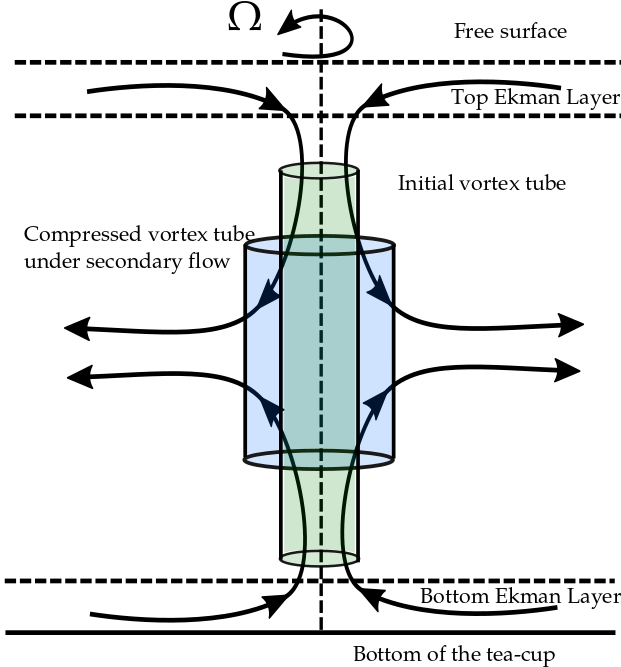
\includegraphics[scale = 0.5]{Figs/tea_cup.png}
    \caption{Compression of vortex tubes under secondary flow set-up due to Ekman pumping in a tea-cup.}
    \label{fig:tea_cup}
\end{figure}
First, we explain why the fluid will be pumped out of the Ekman BLs in the spin-down problem of a tea-cup. In the inviscid interior, the hydrodynamic pressure gradient exactly balances the centrifugal acceleration. This same pressure is impressed into the BL. However, inside the BL, due to no-slip BCs at the bottom, velocities drop dramatically and the hydrodynamic pressure gradient wins over the centrifugal forces. Hence, the flow is `towards' the axis in the bottom Ekman BL. A secondary flow is set-up as shown in Fig.(\ref{fig:tea_cup}) due to continuity. The fluid is pumped out of both BLs at the top and bottom. Under this planar-extension-type flow, an initial thin, long vortex tube is compressed to a fat, short one as shown indicated in Fig.(\ref{fig:tea_cup}). Since the flow in the interior is inviscid, angular momentum is conserved. To compensate for the compressed vortex tubes the flow must slow down in order to conserve angular momentum. Spin-down happens for this reason. \\
%
Now, considering Eqn.(\ref{eq:qg-vort-eqn-2}), neglecting the $\beta$ plane effects as well as the advective nonlinearity, we attempt to find the time-scale of spin-down. 
\begin{equation}
 \pd{\omega_{z0}}{t} = - \frac{r}{\sqrt{2}}\omega_{z0} 
\end{equation}

$\omega_{z0} = \omega_{z0}(0)e^{-t/T}$, with $T = \frac{\sqrt{2}}{r} = \frac{\sqrt{2}\epsilon}{\sqrt{E}}$. Dimensionally, $T = \frac{\sqrt{2}\epsilon}{\Omega\sqrt{E}}$. Writing $E = \nu/f_{0}D^{2} = \frac{\nu}{2\Omega D^{2}}$ and $\epsilon = U_{0}/Lf_{0} \approx 1/2$. Giving, $T = \frac{\sqrt{2}\cdot (1/2)}{\Omega \cdot \frac{\sqrt{\nu}}{\sqrt{2\Omega}D}}  = \frac{D}{\sqrt{\Omega \nu}}$. For typical values, $D = 4$ cm, $\Omega = 2\pi$, $\nu = 10^{-2} \textrm{cm}^{2}\textrm{s}^{-1}$, we get $T \approx 20$s, a good approximation that matches with day-to-day experience!

%------------------------------------------------------
\bibliographystyle{apalike}
%\bibliographystyle{unsrt} % Use for unsorted references  
%\bibliographystyle{plainnat} % use this to have URLs listed in References
%\cleardoublepage
%\bibliography{References/references} % Path to your References.bib file

\bibliography{bib/references} % Path to your References.bib file
 \if@openright\cleardoublepage\else\clearpage\fi
 \cleardoublepage
 \pagestyle{empty}
%--------------------------------------------------------------------
\end{document}
